\documentclass[pageno]{jpaper}

%replace XXX with the submission number you are given from the ISCA submission site.
\newcommand{\IWreport}{ 2013}
\doublespacing
\usepackage[normalem]{ulem}
\usepackage{amsmath}
\usepackage{graphicx}
\usepackage{tikz}
\tikzset{>=latex}
\graphicspath{ {./Graphs/} }
\begin{document}

\title{Authorship Attribution on Twitter: A Comparative Methods Study}
\author{Author: Julian Griggs (jgriggs@princeton.edu) \\ Advisor: Andrea LaPaugh (aslp@cs.princeton.edu)}
\date{}
\maketitle

\thispagestyle{empty}

\begin{abstract}
\label{sec:abstract}
Stylometric analysis is becoming an increasingly powerful tool for de-anonymizing written texts on the web.     Despite the large growth in social media based text, authorship attribution studies focusing on this domain are relatively scarce.  In this paper, I analyze the effectiveness of some of the most commonly used linguistic features and machine learning algorithms to quantitatively determine the best combination for authorship attribution in the Twitter domain.  Empirical data suggests that across the feature-analysis method combinations tested, pairing Character 2-grams with Linear Support Vector Machines yields the best overall performance.
\end{abstract}

\section{Introduction}
\label{sec:intro}
Communication in the world today is very different from that of 25 years ago.  25 years ago was around the time when personal computers first became affordable, the internet was just beginning to popularize, and the use of emails and mobile phones were on the horizon.  Fast forward to the present day and the differences are truly staggering.  Today, roughly 91\% of Americans own a cell phone \cite{cellphone-ownership},  social networking sites like Twitter transmit over 400 million messages a day \cite{twitterTurns7}, and in some nations such as England, texting is the dominant form of communication \cite{textingFreq}.  With many other forms of digital communication in popular use such as email, blogs, and chatrooms, it cannot be denied that we live in an age marked by digital correspondence.  These streams of communication provide people with many benefits in terms of speed, convenience, and volume; however, such technologies are not without certain dangers.

The extreme growth and adoption of technology for benevolent means has also lead to an increase in its malevolent uses, i.e.  cyber-crime.  Cyber-crime is a serious problem with many of its most common forms including spam, phishing, and cyber-bullying occurring on the very same communication platforms that dominate (email, text messages, social media).  Detecting the culprits of cyber-crime is a problem made challenging by the relative ease with which individuals using these mediums can hide their identities behind pseudonyms such as screen names.  When compounded with the use of anonymity networks such as Tor, the problem becomes even more difficult.  However, when 16\% of high school aged students every year are victims of cyberbullying \cite{Cyberbullying}, 33\% of internet-related sex crimes are instigated through social media \cite{socialmedia-crime}, and with phishing attacks increasing exponentially and moving into new channels of communication \cite{phishing}, something must be done to try to fight back against such crime.

One mechanism aimed at ebbing the flow of online crime is computational stylometry.  Stylometric analysis involves identifying and quantifying various linguistic features present in a written text so as to provide a computational profile of that body of writing.  The power behind this technique comes from the fact that writing styles are very often unique enough to distinguish one author from another.  Therefore, computational stylometry makes the task of grouping anonymous texts together by author quite possible in many contexts.  Once a group of texts is shown to be linked stylistically, if the author of one such text in the group is known, then the anonymity of all other texts linked to it becomes jeopardized.  With so much cyber communication being publicly available, it is conceivable for a message sent in one context to de-anonymize a message sent in another.  Someone's Facebook post could be used to determine the identity of an anonymous cyber bully.  Someone's text message could identify the author of a phishing email.  It is exactly these types of cross-context linkages that lend so much power to the domain.

The goals of this study are to:
\begin{itemize}
\item{show that given enough training data, machine learning and stylometry can be used to determine authorship of twitter data.}
\item{quantify the best feature-analysis method pairing for stylometry as applied to Twitter data.}
\item{determine how accuracy of the authorship attribution task changes with increasingly large training and test documents, as well as increasingly sized pools of potential authors.}
\item{gain insight into whether the authorship attribution task is complicated by using authors that belong to similar domains (Musicians, Athletes, Entertainers, etc.)}
\end{itemize}

\section{Background}
\label{sec:background}

\subsection{What is Stylometry}
\label{sec:whatIsStylometry}
As it is commonly defined, stylometry is a discipline that uses statistical analysis and machine learning to quantify and then classify written texts according to various properties.  One of the most common uses of stylometry is its application to authorship attribution: determining the author of an unknown text from a pool of candidate authors.  Authorship attribution has been used throughout history in authorship disputes involving  the works of Shakespeare, the Federalist Papers, and recently, it was used to reveal J.K. Rowling as the true author of the critically acclaimed novel \underline{The Cuckoo's Calling} which she published under a pseudonym.  You might wonder, how does authorship attribution work, anyhow?  The answer is that it combines the selective extraction of representative, linguistic features from a text with a choice of the model used to analyze them.  In other words, the human component of this process is merely to determine which linguistic features should be allowed to be extracted, while it is the job of the machine learning algorithm to tailor its use of these specified features appropriately.
\label{sec:authorship-attribution}

\subsection{Feature Set}
\label{sec:featureSet}
Generally speaking, the features characteristic of any piece of text fall into a few broad categories: lexical, syntactic, and application-specific.
\subsubsection{Lexical}
\label{sec:lexical}
\indent \\
Lexically defined features are those that relate to the actual words present in a given piece of text.  The most commonly used lexical features are: word length, sentence length, vocabulary richness, punctuation frequencies, word/character frequencies, and word/character n-grams \cite{survey}.  For the entirety of a document, the character length of each word and of each sentence is measured and then averaged giving a basic quantitative measure of a piece's complexity.  These features have the benefit that they can be readily applied to any language \cite{survey} but may be extremely dependent upon context.  Vocabulary richness is defined by the the number of unique words, $U$, divided by the total number of words, $W$.  However, as Stamatos points out, this measure is highly dependent on the length of the text(with shorter texts generally having a more diverse spread of words) thus this feature when used alone is unreliable \cite{survey}.  Word frequency is a very common metric, that is oftentimes broken up into two categories: "content word" frequency and "function word" frequency.  Content words are those words in a text that carry information about the subject matter while "function words" are word that take on the grammatical roles (articles, pronouns, conjunctions, etc) that allow for properly constructed sentences \cite{performance_of_features}.  Consider, for example, the following quotation from Mark Twain:
\begin{center}"It's not the \underline{size} of the \underline{dog} in the \underline{fight}, it's the \underline{size} of the \underline{fight} in the \underline{dog}." \end{center} In the above quotation, all of the content words are underlined while the function words are left normal.  One issue with the use of this measure is that what constitutes a function word is not well defined with different studies using different word selections.  Despite this issue, the analysis of function word frequency has proven to be one of the most successful in terms of predicting authorship of a text \cite{performance_of_features} with the intuition behind this fact being that function words are closely linked to an author's individual grammar and as such are not likely to be consciously controlled, while at the same time being quite unique across individuals \cite{Argamon05measuringthe}.  Simply determining word and character frequencies doesn't account for the context in which these words are used, thereby leaving out this potentially useful feature.  The use of n-grams corrects for this.  Analysis of word n-grams requires splitting up the text into tokens (words) and then treating every consecutive $n$ tokens as a single token.  Character n-grams are defined the same way with the exception that a token is now a single character.  Consider the same example used before: 
\begin{center} It's not the size of the dog...\end{center}
In this example, the word 3-grams include: 
"Its not the", "not the size", "the size of", "size of the", and "of the dog".
The advantages of using character n-grams is that they account for punctuation as well.
Other lexical features, including spelling errors, flexible patterns(flexible word n-grams) and $k$-signatures (mostly unique character n-grams), exist and are often used, but all other features are in some way modeled off of the one described above.  

\subsubsection{Syntactic}
\label{sec:syntactic}
\indent \\
Syntactically defined features are those that relate to the grammatical structure of a given text.  Such features include: frequency of different Parts-of-Speech (POS), POS n-grams, POS-phrases (noun-phrases, verb-phrases, etc.), punctuation, and grammatical errors \cite{Syntactic-authorship} \cite{survey}.  The use of syntactic features is made more challenging due to the pre-processing involved; a tool must first convert all tokens into their appropriate POS, for example.  Despite, the lack of a perfect, commercial natural language processing (NLP) tool, studies have shown that current tools are effective enough at performing the necessary NLP tasks \cite{Syntactic-authorship}. For the same reason that function words are useful, i.e. they are generally used both systematically and unconsciously by the author \cite{Argamon05measuringthe}; so too are syntactic elements  \cite{survey}.  This supposed unconscious, systematic use of grammatical structures seems highly useful for the task of authorship attribution, however, due to the uniqueness of each language, and the relative difficulty to correctly parse text for grammatical features \cite{survey}, the use of syntactic elements is not as powerful as you would think.  Some studies have found that basic syntactic features alone yield worse performance than their lexical counterparts while in others they have been shown to perform better.  Specifically, one study has shown that syntactic features yield strictly less performance than their lexical counterparts \cite{DBLP:conf/coling/Gamon04} while another study that used more elaborate syntactical analysis schemes has shown them to actually outperform lexical features \cite{Syntactic-authorship}.  Either way, the combined usage of these two types of features generally outperforms the use of only one.

\subsubsection{Application-Specific}
\label{sec:applicationSpecific}
\indent \\
Unlike the previous two feature categories that are independent of the medium the text is presented in (email, academic work, blog), application-specific features, by definition, make use of text-specific meta-information.  Consider Figure \ref{fig:Tweet} which shows an example piece of Twitter data, a Tweet.
\begin{figure}[h!]
\begin{center}
\includegraphics*[scale = .55]{example_Tweet}
\end{center}
\caption{Anatomy of a Tweet}
\label{fig:Tweet}
\end{figure}
\\
Every Tweet object, like the one shown above comes with meta-information including the name and Twitter Handle of the author, the Tweet's text, the number of people who ReTweeted (re-posted) the message, the number of people who Favorited the Tweet, and the time the Tweet was sent.  Conceivably, meta features such as the identity of the people that ReTweeted and/or Favorited a Tweet, in addition to the time the Tweet was sent could be application-specific features that would aid in the task of authorship attribution.  However, since these mechanisms do not directly relate to the textual component of the Tweet, their use will not be explored further.  The application specific features of Twitter data that do relate to the textual component include the use of At-Replies (directed messages marked by '@') and hashtags (marked by '\#').  Both of these features are very specific to, and heavily present in, Twitter data.  As such, the analysis of these features, including frequency, length, etc. would provide useful in the quantitative characterization of the text

\subsection{Analytic Models}
\label{sec:analysticModels}
The analytic model is what adds the computational and machine learning aspect to modern stylometry, since extracted features are of little use unless they can be used to extrapolate to unseen texts.  Stamatatos (09), explains that analytic models as used for authorship attribution tasks fall into two categories: profile-based and instance-based approaches \cite{survey}.  The main difference between profile-based approaches and instance-based approaches is the way in which they represent training texts: profile-based approaches concatenate all training texts from a given author into a single text while instance-based approaches represent each training text individually \cite{survey}.  These different categories lend themselves to different machine learning algorithms, with profile based approaches lending themselves to probabilistic algorithms such as Markov Chains and the many variations of Naive-Bayes, while instance-based approaches
lend themselves well to vector space models such as Support-Vector Machines \cite{survey}.  A thorough analysis of all these various methods is outside the scope of this research but as such methods have been heavily studied, further information is easily available.

\section{Related Work}
\label{sec:relatedWork}
This study is not the first to apply authorship attribution methods to Twitter data.  A 2010 study by Layton et. al tested the effectiveness of the profile-based Source Code Authorship Profile (SCAP) methodology in its application to the realm of Twitter.  The SCAP method proceeds as follows:
\begin{enumerate}
\item{Concatenate all training documents per author into a single document}
\item{Calculate the top $L$ most frequent character n-grams where $L$ is an integer chosen so as to optimize effectiveness.}
\item{The author with the highest intersection of common n-grams with the test document is the likely author.}
\end{enumerate}
They determined that the SCAP methodology was 70\% effective at determining authorship from a pool of 50 authors, lending credence to the notion that authorship attribution is more than feasible for Twitter Data.  Also of interest, they found that the Twitter specific features, hashtags and At-replies have significant value in the authorship attribution task with up to 27\% accuracy lost when these features were removed \cite{140}.

In general, the study of authorship attribution uses large sized training data in addition to large sized test data.  In the online context however, where messages are commonly quite short, to assume the availability of lengthy textual data is unreasonable.  A study by MacLeod et. al sought to address this issue by determining whether it was possible to determine authorship of a single Tweet (with maximum 140 characters).  They found that by training on 100 Tweets for each of the 20 authors in their sample, correct authorship was determined about 50\% of the time, much higher than the 5\% that would be expected via chance.  However, they found that by aggregating Tweets used for testing, accuracy increased \cite{whose-Tweet}.  Though promising, these results were on a relatively small scale in that they only tested 10 separate Tweets.  Further, their results were not cross validated, thus requiring more trials to ensure validity.  

A number of other studies have been done that have contributed to the knowledge regarding effective features to extract and use for authorship attribution.  It has been shown that for Greek Twitter data, the use of an Author's Multilevel N-gram Profile (a hierarchical combination of word and character n-grams that capture different linguistic features) outperforms the use of any single n-gram feature \cite{Greek-paper}.  This implies that each level of linguistic features(phonology, morphology, and semantics) add value to the authorship attribution task.  The use of $k$-Signatures, n-grams that are unique to an author while also occurring in at least $k$\% of their own Tweets(where $k \in[2, 50]$), has been shown to be relatively common in real Twitter data which helps to explain why authorship-attribution is even possible in this context \cite{schwartz-EtAl:2013:EMNLP}.  Scwartz et. al, also proposed the use of a feature known as a Flexible Pattern to attain additional accuracy in authorship-attribution of micro-messages.  Flexible Patterns are word sequences that begin and end with a high frequency word while containing at least one content word in between them.  The use of flexible patterns, when combined with word and character n-grams was shown to increase attribution accuracy by 6.1\% from 55.5\% to 61.6\% \cite{schwartz-EtAl:2013:EMNLP}.

\section{Methodology}
\label{sec:methodology}

\subsection{Data Retrieval}
\label{dataRetrieval}
The Twitter data used in this study was gathered from publicly visible accounts that Twitter algorithmically designated as being "popular".  There were two main reasons for selecting this data source with the first being logistical and the second being its role in the experiment design: 
\begin{enumerate}
\item{The public nature of these profiles allows for easy Tweet extraction using open-source tools (Twitter4J).}
\item{When Twitter adds an account to its list of "Popular Accounts" they fit the account into a designated category, with each category containing similar users.}
\end{enumerate}
According to Stamatatos, "[a]ny good evaluation corpus for authorship attribution should be controlled for genre and topic."\cite{survey}
Tweets, by their very nature, are on diverse topics even when written by the same author.  Thus, the gathering of a perfectly controlled corpus of Twitter data is not feasible as the medium is inherently not set up along the lines of genre and topic.  However, my choice to gather data from users that fall into specific categories, actually provides this study with some degree of topic control over the corpus used since authors in the same category presumably have some degree of similarity in their interests.
For every user, in each one of the Twitter determined categories, their most recent 1600 Tweets along with metadata including the timestamp, the language of the Tweet, and whether the Tweet was a "reTweet", were extracted using the Twitter4J \cite{twitter4j} library that provides access to the Twitter API.  This resulted in a total of 2,452,800 Tweets gathered from 1533 users spanning across 28 categories.  All Tweets were then filtered so as to remove all URLs and At-replies found within their text bodies.  The decision to remove URLs was mainly due to the fact that URL text cannot be altered by an author stylistically and thus conveys little in terms of stylistic evidence.  This compounded with the fact that Twitter puts their own URL wrapper around all posted URLs, really negates all value that their analysis would serve.  The decision to remove At-replies was made because, without doing so, part of the authorship attribution task would become a social network analysis, thus taking away from the stylometric component that was the focus of this study.

\subsection{Test Parameters}
\label{sec:testParameters}
This study seeks to determine which of the standard set of stylistic features and evaluation methods are best at determining authorship for Twitter data.  The set of features that will be tested are those that are most widely used including: character N-grams, word N-grams, POS N-grams, Mosteller-Wallace function words \cite{MWFunction}, average word length, average sentence length, and word frequencies.
The evaluation methods that will be examined include one profile based method as well as two instance based methods.  The profile based method is Markov-Chain Analysis, while the instance based methods will include Support Vector Machines (SVM) and Burrows Delta.

The performance of every authorship attribution tasks is effected by four parameters: the size of the training corpus, the size of the test corpus, the number of potential authors, and the relative balance or imbalance of texts in the training corpus over the set of candidate authors \cite{survey}.  Since Twitter profiles were chosen categorically, this study will treat Category as a fifth parameter.  Since all of these factors effect the success rate of attributing authorship, this study tests the variation of each of the listed factors, with the exception of training set imbalance which will be left for future study.

\subsection{Experimental Set-Up}
\label{sec:experimentalSetUp}
This experiment is multilayered with the features-evaluation test being the primary study while auxiliary tests regarding the size of the training and test sets, as well as the number of potential authors, are layered on top with every test being done per Twitter category.  The core authorship attribution experiment is made by possible through use of the Java Graphical Authorship Attribution Program (JGAAP), an open-source package created by the Evaluating Variation in Language Laboratory \cite{JGAAP}.   This package provides both a graphical and a command line interface for performing custom authorship attribution experiments.  I will give brief descriptions of all experimental layers with Figure \ref{fig:experimentStructure} being a reference diagram.
\begin{figure}[h!]
\begin{center}
\includegraphics*[scale=.5]{experimentStructure}
\end{center}
\caption{Experimental Structure}
\label{fig:experimentStructure}
\end{figure}
\subsubsection{Core Experiment} 
\label{sec:coreExperiment}
\indent
\\
\textbf{Goal:} Measure performance of each combination of evaluation method with stylistic feature on the attribution of authorship to twitter data.
\\
\textbf{Method:} Given a set of $N$ authors, use random sampling to create training sets of size $M$ Tweets for each author and then choose 5 random authors from this set for which to create a test set according to the size parameters that will be described subsequently.  For every combination of evaluation method and stylistic feature, the classifier will use the training data to guess the authorship of each of the $5$ test sets.  Repeat 5 times.
\subsubsection{Vary Training Set and Test Set Sizes}
\label{sec:varyTrainingAndTest}
\indent
\\
\textbf{Goal:} Determine to what extent changes in the size of the training set and test set effect authorship attribution accuracy.
\\
\textbf{Method:} 
\begin{enumerate}
\item{Perform the Core Experiment described above for increasingly large training documents per author.  The sizes will be 50, 100, 200, and 500 Tweets per author.}
\item{For each training set size, use test sets of increasingly large sizes.  The sizes will be 1, 5, 25, 50, and 100 Tweets concatenated together forming one test document.}
\end{enumerate} 
\subsubsection{Vary Number of Potential Authors} 
\label{sec:varyAuthors}
\indent
\\
\textbf{Goal:} Determine how the efficacy of authorship attribution changes as the number of potential authors varies.
\\
\textbf{Method:} Perform the Core Experiment described above for increasingly large pools of candidate authors.  The sizes will be 5, 10, 25, and 50 authors.

\section{Results}
\label{sec:results}
Due to the complexity of the experimental design (6 different variables: analysis method, feature, category, number of authors, size of training set, size of test set), I will first present some general findings before exploring some of the interesting specifics.
\subsection{General Results}
\label{sec:generalResults}
The first aim of this study was to determine which feature-analysis method pairings are best at the authorship attribution task.  Figure \ref{fig:GeneralResults} shows the performance of all feature-analysis method combinations averaged across all other variables.  
\begin{figure}[h!]
\begin{center}
\includegraphics*[scale=.85]{GeneralFeatureMethodResults}
\end{center}
\caption{Feature-Method Performance Averaged Across Entire Experiment.  See \ref{generalStdDev} to view Standard Deviation data.  See Section \ref{sec:explainingStdDev} for an explanation regarding the magnitudes of the standard deviations.}
\label{fig:GeneralResults}
\end{figure}
Though there does exist some variation when each variable is looked at separately, this graph sums up the general performance of each combination.  From this graph, we determine that overall, the most successful authorship attribution of Tweets comes from extracting Character 2-Grams and using the Linear Support Vector Machines analysis method to perform the machine learning.  Averaged over the entire experiment, this combination correctly predicts the author of an unknown text $79.77\%$ of the time with the runner up being the Parts-of-Speech 2-gram paired again with Linear SVM at $75.03\%$ accuracy.  

Further study of this graph reveals that, in fact, 4 of the top 5 feature-method pairings involve Support Vector Machines.  In fact, if the success rates for each analysis method are averaged across all features, we find that use of Support Vector Machines yield correct authorship attribution $47.76\%$ of the time while Markov Chain Analysis and Burrows Delta have success rates of $29.72\%$ and $23.78\%$ respectively.  Even though Support Vector Machines are the clear winner, all of these numbers are significantly above the expected average of $0.072\%$ (calculated by averaging random selection across each of the different sized author sets tested), lending credence to the real applicability of machine learning to the authorship attribution task.

\subsection{Varying Training Set and Test Set Size}
\label{sec:resultsVaryTrainAndTest}
Also of interest in this study was the determination of how the size of the training set (the number of Tweets known to belong to each author) and the test set (number of Tweets belonging to an unknown author), influence the accuracy of authorship attribution.  Figures \ref{fig:GeneralVaryingTraining} and \ref{fig:GeneralVaryingTest} demonstrate the findings.  
\begin{figure}[h!]
\begin{center}
\includegraphics*[scale=.8]{GeneralVaryingTrainingSetSize}
\end{center}
\caption{How performance of each algorithm varies with the size of each training document.  For data values, see Table \ref{OverallChangeTraining} in the Appendix with Table \ref{trainingStdDev} containing the standard deviation data.  See Section \ref{sec:explainingStdDev} for an explanation regarding the magnitudes of the standard deviations.}
\label{fig:GeneralVaryingTraining}
\end{figure}
\begin{figure}[h!]
\begin{center}
\includegraphics*[scale=.8]{GeneralVaryingTestSetSize}
\end{center}
\caption{How performance of each algorithm varies with the size of each test document.  For data values, see Table \ref{OverallChangeTest} in the Appendix with Table \ref{testStdDev} containing the standard deviation data.  See Section \ref{sec:explainingStdDev} for an explanation regarding the magnitudes of the standard deviations.}
\label{fig:GeneralVaryingTest}
\end{figure}
It turns out that for all three Analysis Methods, the rate of successful authorship attribution increases with the size of the training set as well as the test set.  Intuitively, this makes sense because the more text that is made available to the machine learning algorithms, the more refined their classifications and the more accurate their predictions.  However, this increase is not linear as Figures \ref{fig:GeneralVaryingTraining} and  \ref{fig:GeneralVaryingTest} reveal.  Instead, the graphs are best described as logarithmic with the data revealing that the biggest jumps in attribution accuracy comes from the beginning of the curves i.e increasing the size of the training document from 50 to 100 and increasing the size of the test documents from 1 Tweet to 5.
%**Talk about average number of characters / words a Tweets here ****.  

Also of importance is to note that in Figure \ref{fig:GeneralVaryingTraining} there is no drop in prediction accuracy as the size of the training set increases.  Such a drop would be characteristic of overfitting the machine learning algorithm to the training data.  However, the absence of such a drop is good evidence that up to training documents of size 500 Tweets, all three machine learning algorithms tested are resistant to overfitting.

It is important to note that the conclusions drawn above are based off of data that has been averaged across additional variables.  For example, Figure \ref{fig:GeneralVaryingTest} calculates the prediction accuracy by averaging across all features, author set sizes, and all of the training set sizes.  Thus, before we can be entirely comfortable with the conclusions drawn above, we must look at how these internal factors vary with one another.

Figure \ref{fig:VaryingTest} depicts how the prediction accuracy of the best 3 features for Linear SVMs vary with both test set size and training set size.
\begin{figure}[h!]
\begin{center}
\includegraphics*[scale=.75]{LinearSVMVaryTest50Auth50Train}
\includegraphics*[scale=.75]{LinearSVMVaryTest50Auth500Train}
\includegraphics*[scale=.75]{LinearSVMVaryTest5Auth50Train}
\includegraphics*[scale=.75]{LinearSVMVaryTest5Auth500Train}
\includegraphics*{4graphLegend}
\end{center}
\caption{How performance of each algorithm varies with the size of each test document and the number of authors.}
\label{fig:VaryingTest}
\end{figure}
The juxtaposition of the top-left graph with the top-right graph reveals that for Linear SVMs, the change in prediction accuracy as a function of test set size is roughly equivalent from the smallest training set (the left image) to the largest training set (the right image).  In other words, the impact of test set size is not conditioned on the size of the training set.  When we look at the bottom two graphs, we find that this same relationship holds for author sets of smaller sizes too.  The fact that the same trends are visible with 50 Authors in the test set as well as 5 Authors provides strong evidence that the impact of test set size is not conditioned on the size of the potential set of authors.  This is not to say that prediction accuracy is not influenced, by the number of potential authors.  Rather it explains that the positive correlation between increased test set sizes is present regardless of the size of the set of potential author pool.  If we perform the same analysis, but this time seeing how attribution accuracy varies over the different sized training sets, we find that similarly to the previous case, the impact of training set size is not conditioned on the size of the test  set nor with the number of potential authors.  Reference Figure \ref{fig:GeneralVaryingTrain} in the Appendix for details. It turns out that the very same trends are also seen for the Markov Chain and Burrows Delta analysis methods with Figures \ref{fig:VaryingTestMarkov} and \ref{fig:VaryingTestBurrows} in the Appendix.  These equivalent trends allows us the ability to generalize across multiple variables, as we previously did, because we know that variation across test set sizes, is consistent across different training set sizes, as well as number of authors.  In other words, we can safely assume that the positive correlation we observe between number of Tweets in the test document and the attribution accuracy, when there are 10 potential authors and 500 training Tweets will also exist for 50 authors and 200 training Tweets. 

\subsection{Varying Number of Potential Authors}
\label{sec:resultsVaryAuthors}
Also of interest in this study was the determination of how different feature-analysis method combinations would fare when having to choose an author out of an increasingly large pool of potential authors.  To begin, we will examine how the different analysis methods perform under different author set sizes.  
\begin{figure}[h!]
\begin{center}
\includegraphics*[scale=.85]{GeneralVaryAuthorImprovementOverRandom}
\end{center}
\caption{Accuracy boost analysis method provides over random selection.}
\label{fig:GeneralVaryingAuthorImprovement}
\end{figure}
Figure \ref{fig:GeneralVaryingAuthorImprovement} demonstrates that as the number of authors increases, the accuracy boost over random selection provided by each analysis method decreases, with the largest decrease appearing in the range between 10 potential authors and 25 potential authors in the pool.  What this means is that each analysis method adds a greater boost to accuracy when there are few authors as opposed to when there are many.  However, the drop off is much smaller than what would be expected as compared to the way in which random selection false off. Table \ref{percent-change} shows the percent change in the accuracy boost provided by each analysis method from 5 Authors to 50 Authors in comparison to random selection.
\begin{table}[h!]
\centering
\begin{tabular}{|l|l|l|l|}
\hline
                 & 5 Authors & 50 Authors & Percent Change \\ \hline
Markov Chain     & 0.2376    & 0.1708     & -28\%          \\ \hline
Linear SVM       & 0.4561    & 0.296      & -35\%          \\ \hline
Burrows Delta    & 0.186     & 0.1053     & -43\%          \\ \hline
Random Selection & 0.2       & 0.02       & -90\%          \\ \hline
\end{tabular}
\caption{Percent Change in Analysis Method vs. Random}
\label{percent-change}
\end{table}
All analysis methods turn out to be at least twice as robust to increased sized author sets as random selection with Markov Chain analysis actually proving to be the most robust, followed by Linear SVM. 

Going one level deeper, we now observe how the top 3 features for each analysis method respond to changes in the number of authors. 
\begin{figure}[h!]
\begin{center}
\includegraphics*[scale=.5]{Top3Markov}
\includegraphics*[scale=.5]{Top3SVM}
\includegraphics*[scale=.5]{Top3BurrowsDelta}
\includegraphics*[scale=.9]{featureLegend}
\end{center}
\caption{How feature-method pairs perform as number of authors increases (500 Tweets in Training Set and 100 Tweets in Test Set)}
\label{fig:FeaturesVaryingAuth}
\end{figure}
Figure \ref{fig:FeaturesVaryingAuth} demonstrates that all 3 analysis methods have a feature that when paired with, enables authorship prediction rates very near 100\% at the 5 author level.  In fact, Markov Chain analysis and Linear SVMs make it all the way to the 25 author mark while maintaining a feature pairing that predicts authorship near perfectly.  At the 50 author mark, the overall best feature-analysis method pairing is Character 2-grams with Linear SVMs which correctly predicts authorship 89.6\% of the time.  An interesting, and unexpected, result is that different analysis methods better utilize different features.  For example, the best feature for Linear SVMs is Character 2-grams while the best feature for Markov Chain Analysis is word frequency.  Furthermore, we can see that the instance based approaches (Linear SVM and Burrows Delta) have a few best-features in common, while having no overlap with the best features for Markov Chain Analysis.  Further research would go into understanding the reasons for these differences.

\subsection{Standard Deviations Explained}
\label{sec:explainingStdDev}
We have now observed enough to explain the large standard deviations for the data displayed in Figures \ref{fig:GeneralResults}, \ref{fig:GeneralVaryingTraining}, and \ref{fig:GeneralVaryingTest}.  At first glance, the fact that the standard deviation data is on the same order of magnitude as the averages, seems to be an alarming fact that would signal unreliable data.  However, these large standard deviations are in fact expected, given the way the data is displayed.  Remembering that Figures \ref{fig:GeneralResults}, \ref{fig:GeneralVaryingTraining}, and \ref{fig:GeneralVaryingTest} display the average authorship attribution rates averaged across all other variables, it makes sense that variations in the other variables would cause large standard deviations.  For example, as we have already shown in Table \ref{percent-change}, variation in the number of authors can lead to large differences in the attribution success rate.  Variations in the size of the training and test sets affect the raw attribution rate on an even greater scale.  Thus when one looks at the raw standard deviation values as shown in Tables \ref{generalStdDev}, \ref{trainingStdDev}, and \ref{testStdDev}, it is important to remember that large values are to be expected.

\subsection{Varying Across Categories}
\label{sec:categories}
Though not of express interest to this study, the experimental design was such that it allowed for comparisons of authorship attribution rates across the 5 different categories tested.  What the data shows is that for all 3 of the analysis methods, the authorship attribution rates seem to be more or less consistent across all categories.  Specifically, the features best at predicting authorship in one category tend to be the same features that are best in all other categories.  This trend holds most strongly for the best features, with some variation being seen for lower ranked features, probably as a result of their success rates being the closest together and thus most affected by small random variations.  Complete figures are included in the Appendix.
\subsection{Comparison to Previous Results}
\label{sec:comparison}
My results are on par with previous studies into authorship attribution on Twitter data.  As described earlier the SCAP methodology, as used by Layton et. al was 70\% effective at determining authorship from a pool of 50 authors.  My data shows that, when averaging over all test and training set sizes, the best feature-method pair (Character 2-grams with Linear SVM) correctly predicts authorship at the 50 author level with the same accuracy.  Since the SCAP methodology also extracts N-gram features, it can be said that the Simplified Profile Intersection distance metric used in the SCAP experiment utilizes N-Gram features just as well as Linear SVMs to attribute authorship.  However, the Layton et. al study performed authorship attribution experiments by grouping randomly aggregated Twitter users, spanning across multiple different domains.  This differs from my study where all tests are done with users that come from the same Twitter Category/domain.  Intuitively, one would imagine that users belonging to the same Twitter Category would have  Tweets about similar topics, and thus less differentiable writing styles than a group of randomly selected users.  This intuition would imply that the Character 2-gram-Linear SVM combination would in fact perform better than 70\% on the dataset used in Layton et. al.  In order to begin exploring this path, I simply ran the Linear SVM portion of this experiment on a collection of user selected uniformly at random across all Twitter categories.  The results are displayed fully in Table \ref{table:randAuthorSets}, however the general summary according to this preliminary test is that our intuition is not correct.  It does not appear that the authorship attribution task is made more complex, on the whole, by having topically similar authors in the set of potential candidates.  Future research would go into exploring this possible dichotomy in greater depth.
\begin{table}[h!]
\centering
\begin{tabular}{|l|l|l|}
\hline
                & Authors Across Categories & Authors Within Categories \\ \hline
Char 2:grams    & 0.63                      & 0.7                       \\ \hline
Char 3:grams    & 0.38                      & 0.39                      \\ \hline
Function Words  & 0.19                      & 0.26                      \\ \hline
POS 2:grams     & 0.23                      & 0.63                      \\ \hline
POS3:grams      & 0.58                      & 0.27                      \\ \hline
Sentence Length & 0.33                      & 0.1                       \\ \hline
Word Length     & 0.31                      & 0.29                      \\ \hline
Word 2-grams    & 0.2                       & 0.07                      \\ \hline
Word 3-grams    & 0.42                      & 0.08                      \\ \hline
Words           & 0.44                      & 0.38                      \\ \hline
\end{tabular}
\caption{Random 50 Author Sets vs. Topically Related 50 Author Sets.  Success rates averaged across all training and test set sizes.}
\label{table:randAuthorSets}
\end{table}

Earlier, I discussed how studies such as \cite{Argamon05measuringthe} and \cite{performance_of_features} determined that in the general case of stylometry, the function words feature is very effective at distinguishing an author's writing style.  My results show that this is less true in their application to the domain of Twitter.  Averaged across the entire experiment, the function words feature ranked 7 out of 10 for both Markov Chains and Linear SVMs, while ranked higher at 4th for Burrows Delta Analysis.  One possible theory to explain this discrepancy is that the language chosen for use in Tweets is not as well grammatically structured as the more formal language that the previous studies looked at, and to a good degree I believe that this is true. However, when function words are used in the setting of large sized training and test sets, their success rates improve significantly, more than doubling from 41.5\% on average to predicting at an accuracy of 83\% when coupled with Linear SVM.  This substantial increase in effectiveness at larger sized training and test sets could provide evidence of an alternative theory that posits the reason for the overall discrepancy is that function word patterns only emerge in larger text corpuses.  Further research would go into putting both of these theories to the test.

To recount, the study by Macleod et. al determined that authorship could be determined with 50\% probability with 20 potential authors, 100 Tweets in each training set, and 1 test Tweet.  By matching these constraints as closely as possible, with the only difference being 25 potential authors as opposed to 20, it turns out that the Character 2-gram-Linear SVM pair again performs the best, correctly predicting authorship with 31\% probability.  The additional 5 potential authors could be part of the reason for the discrepancy from the 50\% mark demonstrated by Macleod et. al but as their study only performed 30 total tests, while my study performed 125 such tests, it is also possible that the inconsistency comes from random variation in their study that persisted due to lack of data.

\section{Conclusion}
\label{sec:conclusion}

Through my research I have encountered many questions and ideas for further study that would be answered by one of four extensions:
\begin{itemize}
\item{Add more machine algorithms as analysis methods}
\item{Experiment with the effectiveness of different combinations of features}
\item{Add more training and test set sizes}
\item{Add more author set sizes}
\end{itemize}
By extending this experiment to include more machine learning algorithms, better insight can be gleaned into why different machine learning algorithms best utilize different linguistic features.  Similarly, this extension would allow more insight into the differences between instance-based and profile-based approaches.  After these differences are better understood, the core part of this experiment could be enhanced so as to begin testing different feature combinations with the various analysis methods.  For example, tests could be done to determine if using Linear SVM with both Character 2-grams and POS 2-grams boosts performance beyond using Character 2-grams alone.
Extending the experiment to include more training and test set sizes would allow you to more closely hone in on the critical point where increasing the size of the training and test documents no longer becomes as beneficial.  Alternatively, the experiment could be modified so that authorship attribution tests were done using training sets that vary in size across authors.  Such a study would reveal how different analysis methods respond to unevenly weighted training data.  Finally, an extension of this study that tests the effectiveness of each feature-analysis method pairing in more extreme conditions, where there may be hundreds or even thousands of authors would more accurately determine the real world applicability of the authorship attribution task in an online context.

%Further explore the effects of user domain on writing style.

I believe that this research has made useful contributions in that it conclusively determines which linguistic features should be paired with which analysis methods for optimal authorship attribution.  Specifically it determines that Character 2-grams paired with Linear SVM analysis yields the best success rates.  In addition, I have determined that success rates do in fact improve over increasingly sized training and test documents, though the marginal benefit decreases as size increases.  I have also shown that the biggest drop in authorship attribution accuracy comes somewhere in the range of 10-25 potential authors, signaling that at some point in this range, the task becomes quantitively more difficult.  Finally, I have shown preliminary evidence that the authorship attribution task is not made more difficult when the potential authors are all members of a common topic group.  Future research would follow up on this to more conclusively determine it validity.
\section{Acknowledgements and Honor Code}
\label{sec:acknowledgements}
First and foremost, I would like to thank my advisor, Andrea LaPaugh, for her guidance throughout my research.
I would also like the JGAAP authors for providing such a fantastic tool.
Also, a special thanks to Efstathios Stamatatos for his work and study in the field of Authorship Attribution.  Stamatatos' writings were an invaluable resource.
\\
\textit{This paper represents my own work in accordance with University regulations.}
\\
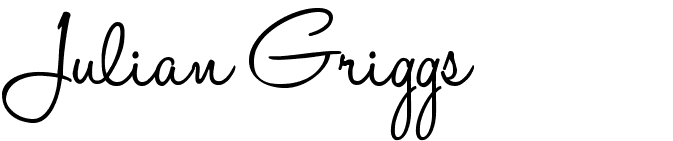
\includegraphics[scale=0.25]{signature}
\bstctlcite{bstctl:etal, bstctl:nodash, bstctl:simpurl}
\bibliographystyle{IEEEtranS}
\bibliography{references}
\section{Appendix}
\begin{table}[h]
\centering
\begin{tabular}{|l|l|l|l|}
\hline
                & Markov Chain & Linear SVM & Burrows Delta \\ \hline
Char 2-grams    & 0.13         & 0.26       & 0.27          \\ \hline
Char 3-grams    & 0.17         & 0.28       & 0.21          \\ \hline
Function Words  & 0.13         & 0.26       & 0.22          \\ \hline
POS 2-grams     & 0.16         & 0.28       & 0.27          \\ \hline
POS 3-grams     & 0.19         & 0.3        & 0.13          \\ \hline
Sentence Length & 0.1          & 0.17       & 0.13          \\ \hline
Word Length     & 0.07         & 0.27       & 0.24          \\ \hline
Word 2:grams    & 0.27         & 0.22       & 0.09          \\ \hline
Word 3:grams    & 0.24         & 0.16       & 0.09          \\ \hline
Words           & 0.25         & 0.29       & 0.12          \\ \hline
\end{tabular}
\caption{Standard Deviations of Prediction Accuracy Across All Variables}
\label{generalStdDev}
\end{table}

\begin{table}[h!]
\centering
\begin{tabular}{|l|l|l|l|l|}
\hline
                      & 50 Tweets   & 100 Tweets   & 200 Tweets  & 500 Tweets \\ \hline
Markov Chain Analysis & 0.273 & 0.289 & 0.311 & 0.316 \\ \hline
Linear SVM            & 0.426 & 0.473 & 0.500 & 0.509 \\ \hline
Burrows Delta         & 0.198 & 0.232 & 0.253 & 0.267 \\ \hline
\end{tabular}
\caption{Overall performance of analysis methods for each training set size}
\label{OverallChangeTraining}
\end{table}

\begin{table}[h]
\centering
\begin{tabular}{|l|l|l|l|}
\hline
                    & Markov Chain & Linear SVM & Burrows Delta \\ \hline
50 Training Tweets  & 0.21         & 0.31       & 0.17          \\ \hline
100 Training Tweets & 0.22         & 0.32       & 0.2           \\ \hline
200 Training Tweets & 0.25         & 0.33       & 0.23          \\ \hline
500 Training Tweets & 0.3          & 0.33       & 0.27          \\ \hline
\end{tabular}
\caption{Standard deviations of overall performance of analysis methods for each training set size.}
\label{trainingStdDev}
\end{table}

\begin{table}[h!]
\centering
\begin{tabular}{|l|l|l|l|l|l|}
\hline
                      & 1 Tweet   & 5 Tweets   & 25 Tweets  & 50 Tweets & 100 Tweets\\ \hline
Markov Chain Analysis & 0.162 & 0.254 & 0.336 & 0.357 & 0.378    \\ \hline
Linear SVM            & 0.215 & 0.362 & 0.549 & 0.602 & 0.66    \\ \hline
Burrows Delta         & 0.108 & 0.158 & 0.266 & 0.31 & 0.348  \\ \hline
\end{tabular}
\caption{Overall performance of analysis methods for each test set size}
\label{OverallChangeTest}
\end{table}

\begin{table}[h]
\centering
\begin{tabular}{|l|l|l|l|}
\hline
                & Markov Chain & Linear SVM & Burrows Delta \\ \hline
1 Test Tweet   & 0.13         & 0.17       & 0.09          \\ \hline
5 Test Tweets   & 0.19         & 0.25       & 0.12          \\ \hline
25 Test Tweets  & 0.26         & 0.31       & 0.21          \\ \hline
50 Test Tweets  & 0.28         & 0.31       & 0.24          \\ \hline
100 Test Tweets & 0.29         & 0.31       & 0.27          \\ \hline
\end{tabular}
\caption{Standard deviations of overall performance of analysis methods for each test set size.}
\label{testStdDev}
\end{table}

\begin{figure}[h!]
\begin{center}
\includegraphics*[scale=.75]{LinearSVMVaryTrain50Auth25Test}
\includegraphics*[scale=.75]{LinearSVMVaryTrain50Auth100Test}
\includegraphics*[scale=.75]{LinearSVMVaryTrain5Auth25Test}
\includegraphics*[scale=.75]{LinearSVMVaryTrain5Auth100Test}
\includegraphics*{4graphLegend}
\end{center}
\caption{How performance of each algorithm varies with the size of each training document and the number of authors.}
\label{fig:GeneralVaryingTrain}
\end{figure}

\begin{figure}[h!]
\begin{center}
\includegraphics*[scale=.75]{A1}
\includegraphics*[scale=.75]{A3}
\includegraphics*[scale=.75]{A2}
\includegraphics*[scale=.75]{A4}
\end{center}
\caption{How performance of each algorithm varies with the size of each test document and the number of authors.}
\label{fig:VaryingTestMarkov}
\end{figure}

\begin{figure}[h!]
\begin{center}
\includegraphics*[scale=.75]{B1}
\includegraphics*[scale=.75]{B3}
\includegraphics*[scale=.75]{B2}
\includegraphics*[scale=.75]{B4}
\end{center}
\caption{How performance of each algorithm varies with the size of each test document and the number of authors.}
\label{fig:VaryingTestBurrows}
\end{figure}

\begin{figure}[h!]
\begin{center}
\includegraphics*[scale=.75]{MarkovBusiness}
\includegraphics*[scale=.75]{MarkovEntertainment}
\end{center}
\label{fig:MarkovCategories1}
\end{figure}

\begin{figure}[h!]
\begin{center}
\includegraphics*[scale=.75]{MarkovMusic}
\includegraphics*[scale=.75]{MarkovSports}
\end{center}
\label{fig:MarkovCategories2}
\end{figure}

\begin{figure}[h!]
\begin{center}
\includegraphics*[scale=.75]{MarkovTelevision}
\includegraphics*[scale=.75]{MarkovAll}
\end{center}
\label{fig:MarkovCategories3}
\end{figure}

\begin{figure}[h!]
\begin{center}
\includegraphics*[scale=.75]{SVMBusiness}
\includegraphics*[scale=.75]{SVMEntertainment}
\end{center}
\label{fig:SVMCategories1}
\end{figure}

\begin{figure}[h!]
\begin{center}
\includegraphics*[scale=.75]{SVMMusic}
\includegraphics*[scale=.75]{SVMSports}
\end{center}
\label{fig:SVMCategories2}
\end{figure}

\begin{figure}[h!]
\begin{center}
\includegraphics*[scale=.75]{SVMTelevision}
\includegraphics*[scale=.75]{SVMAll}
\end{center}
\label{fig:SVMCategories3}
\end{figure}

\begin{figure}[h!]
\begin{center}
\includegraphics*[scale=.75]{BDBusiness}
\includegraphics*[scale=.75]{BDEntertainment}
\end{center}
\label{fig:BDCategories1}
\end{figure}

\begin{figure}[h!]
\begin{center}
\includegraphics*[scale=.75]{BDMusic}
\includegraphics*[scale=.75]{BDSports}
\end{center}
\label{fig:BDCategories2}
\end{figure}

\begin{figure}[h!]
\begin{center}
\includegraphics*[scale=.75]{BDTelevision}
\includegraphics*[scale=.75]{BDAll}
\end{center}
\label{fig:BDCategories3}
\end{figure}

\end{document}
